\begin{frame}{Allgemeines}
    \begin{columns}[T] % T aligns the tops of the columns
        \begin{column}{0.55\textwidth}
            \vspace*{0.2cm}
            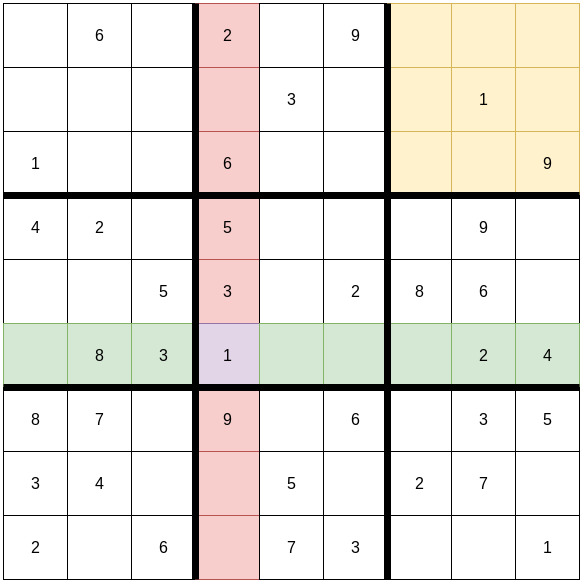
\includegraphics[width=\textwidth]{Pictures/Leer.png}
        \end{column}
        \begin{column}{0.55\textwidth}
            \begin{itemize}
                \item 9x9 Gitter mit Zahlen von 1 bis 9
                \item leere Felder so ausfüllen, dass jede Zahl in
                jeder Zeile, jeder Spalte und jedem 3x3-Block genau 1-mal vorkommt
                \item verschiedene Schwierigkeitsgrade in Abhängigkeit von Anzahl 
                gegebener Felder
                \item weitere Varianten wie z.B. 25x25
                \item BruteForce: \(9^{41}=1.3\cdot 10^{39}\) - \(9^{64}=1,2\cdot 10^{61}\) Möglichkeiten (abhängig von Schwierigkeit)
            \end{itemize}
        \end{column}
    \end{columns}
\end{frame}